% ----------------------------------------------------------
% Experimentos e Discussão dos Resultados
% ----------------------------------------------------------
\chapter{Experimentos e Discussão dos Resultados}

Este capítulo apresenta e discute os resultados em duas frentes. Primeiro, caracteriza-se o conjunto de dados sintéticos gerado, verificando a aderência das distribuições realizadas às fontes estatísticas que as fundamentam, a coerência dos cenários de contraste e a sensibilidade do problema ao componente idiossincrático do gerador. Em seguida, apresentam-se os resultados da modelagem preditiva com os classificadores \textit{Decision Tree}, \textit{Random Forest} e XGBoost frente aos \textit{baselines} de referência, contemplando o estudo de ablação das variáveis derivadas, a comparação de métricas nos conjuntos de \textit{holdout} e validação cruzada ($k=10$) com verificação estatística das diferenças, a análise por classe via curvas ROC e matrizes de confusão, e a interpretação da importância dos atributos.

\section{Caracterização da Base Sintética e Aderência às Fontes}

O conjunto de dados definitivo contém 3.000 registros gerados sob o cenário base (rede pública estadual do Piauí), com semente aleatória fixa para reprodutibilidade. A Tabela~\ref{tab:aderencia} compara, para os principais parâmetros, o valor-alvo derivado das fontes com o valor efetivamente realizado na base gerada.

\begin{table}[htb]
\centering
\caption{Aderência entre os parâmetros-alvo (fundamentados nas fontes) e as distribuições realizadas na base sintética.}
\label{tab:aderencia}
\begin{tabular}{p{6cm}cc}
\toprule
\textbf{Indicador} & \textbf{Alvo} & \textbf{Realizado} \\
\midrule
Renda \textit{per capita} até 0,5 SM & 60,0\% & 58,0\% \\
Acesso doméstico à internet & 92,5\% & 92,6\% \\
Posse de computador ou \textit{tablet} & 25,5\% & 26,1\% \\
Estudantes trabalhadores & 26,3\% & 27,3\% \\
Distorção idade-série & 21,7\% & 22,7\% \\
\bottomrule
\end{tabular}
\source{Elaborado pelo autor (2026).}
\end{table}

Todas as distribuições realizadas situam-se a menos de dois pontos percentuais dos alvos documentados, atestando a fidelidade da parametrização. A distribuição etária apresenta a assimetria positiva esperada (coeficiente de assimetria de $+1{,}39$; mediana de 16 anos; máximo de 24), reproduzindo a cauda longa da distorção idade-série em vez de uma distribuição normal artificial. A regra de elegibilidade do Pé-de-Meia resultou em 47,7\% de beneficiários efetivos (coerente com um cenário em que 58\% dos estudantes se encontram na faixa de renda elegível e a adesão é de 85\% condicionada à frequência mínima). As variáveis acadêmicas parciais do primeiro semestre apresentaram médias plausíveis para o contexto: nota média de 6,4; frequência média de 84,8\%; média de 5,9 nas atividades, com taxa de entrega de 63,8\%; e 0,62 reprovação acumulada por estudante.

A variável-alvo, rotulada pelos critérios da LDB sobre a projeção anual (média mínima de 6,0 e frequência mínima de 75\%, com banda pedagógica de fronteira para a classe intermediária), distribuiu-se em 45,0\% de \textit{Aprovados}, 31,7\% \textit{Em Risco} e 23,3\% de \textit{Reprovados}. Destaca-se que essas proporções \textbf{emergem} da regra de rotulagem (não foram calibradas por limiares de distribuição), e configuram um desbalanceamento moderado e realista, no qual nenhuma classe é dominante, justificando o emprego do SMOTE no treinamento.

Nos cenários de contraste, o gerador comportou-se de forma coerente. No perfil de \textbf{média nacional}, as classes distribuíram-se em 46,7\% / 30,1\% / 23,1\%, próximas do cenário base (consistente com o fato de os indicadores piauienses de conectividade e distorção se aproximarem das médias nacionais após as políticas recentes). No perfil de \textbf{alta vulnerabilidade}, a proporção de reprovados subiu para 36,0\% e a de beneficiários do Pé-de-Meia alcançou 57,6\%. No perfil de \textbf{rede privada de renda alta}, 81,4\% dos estudantes projetam-se aprovados e apenas 6,5\% tornam-se beneficiários (resultado emergente exclusivamente da regra de elegibilidade, sem qualquer parâmetro dedicado, o que confirma a hipótese H4).

\section{Sensibilidade ao Ruído Idiossincrático}

Como descrito na Metodologia, a deriva do segundo semestre possui um componente idiossincrático (ruído gaussiano que representa os fatores não observáveis, como saúde, eventos familiares e motivação, capazes de alterar trajetórias escolares). O parâmetro \texttt{NOISE\_LEVEL} controla a magnitude dessa variância e, por consequência, o teto teórico de acurácia alcançável por qualquer classificador (erro de Bayes do problema). Para caracterizar essa relação, o desempenho da \textit{Random Forest} (hiperparâmetros fixos, validação cruzada estratificada $k=5$ com SMOTE no \textit{fold}) foi medido sob diferentes níveis de ruído, mantidos constantes todos os demais parâmetros (Tabela~\ref{tab:ruido}).

\begin{table}[htb]
\centering
\caption{Análise de sensibilidade: desempenho da \textit{Random Forest} em função da variância idiossincrática do gerador.}
\label{tab:ruido}
\begin{tabular}{cccc}
\toprule
\textbf{\texttt{NOISE\_LEVEL}} & \textbf{$\sigma$ da média (pontos)} & \textbf{$\sigma$ da frequência (p.p.)} & \textbf{Acurácia (CV $k$=5)} \\
\midrule
0,0 & 0,00 & 0,0 & 90,7\% $\pm$ 0,8\% \\
1,0 & 0,10 & 0,8 & 90,2\% $\pm$ 0,6\% \\
2,0 & 0,20 & 1,6 & 88,1\% $\pm$ 0,8\% \\
\textbf{3,0} & \textbf{0,30} & \textbf{2,4} & \textbf{84,3\% $\pm$ 0,6\%} \\
4,0 & 0,40 & 3,2 & 80,5\% $\pm$ 1,6\% \\
5,0 & 0,50 & 4,0 & 77,5\% $\pm$ 1,2\% \\
6,0 & 0,60 & 4,8 & 74,4\% $\pm$ 1,2\% \\
8,0 & 0,80 & 6,4 & 68,7\% $\pm$ 1,4\% \\
\bottomrule
\end{tabular}
\source{Elaborado pelo autor (2026).}
\end{table}

A curva evidencia a degradação monotônica do desempenho com o aumento da variância não observável, confirmando que os classificadores não memorizam a regra geradora, apenas aproximam o sinal observável. Ressalta-se que a varredura \textbf{caracteriza o problema}, não busca uma acurácia-alvo: o valor adotado na base definitiva (\texttt{NOISE\_LEVEL} $= 3{,}0$, equivalente a um desvio-padrão de 0,3 ponto na média anual projetada e de 2,4 pontos percentuais na frequência) é uma decisão fenomenológica, registrada na matriz de rastreabilidade, que representa uma magnitude plausível de variação semestral atribuível a fatores idiossincráticos. Sob essa escolha, o desempenho esperado situa-se na faixa de 80--85\%, compatível com os resultados reportados pela literatura de EDM em problemas análogos \cite{costa2012, shabnam2025}.

\section{Estudo de Ablação das Variáveis Derivadas}

Antes da comparação final, avaliou-se a contribuição de cada variável derivada candidata por meio de um estudo de ablação (validação cruzada estratificada $k=10$, SMOTE no \textit{fold}, hiperparâmetros fixos moderados). A Tabela~\ref{tab:ablation} resume as configurações principais.

\begin{table}[htb]
\centering
\caption{Estudo de ablação das variáveis derivadas (acurácia média na validação cruzada, $k=10$).}
\label{tab:ablation}
\small
\begin{tabular}{p{5.4cm}ccc}
\toprule
\textbf{Configuração} & \textbf{\textit{Decision Tree}} & \textbf{\textit{Random Forest}} & \textbf{XGBoost} \\
\midrule
Sem variáveis derivadas & 80,1\% & 84,9\% & 84,5\% \\
+ \texttt{nota\_x\_frequencia} & 80,9\% & 84,7\% & 84,7\% \\
+ \texttt{reprov\_por\_serie} & 80,3\% & 84,7\% & 84,5\% \\
+ escore acadêmico composto & 79,6\% & 84,2\% & 84,1\% \\
Conjunto final (duas derivadas) & 79,7\% & 84,6\% & 84,9\% \\
Conjunto final + escore composto & 80,2\% & 84,5\% & 84,9\% \\
\bottomrule
\end{tabular}
\source{Elaborado pelo autor (2026).}
\end{table}

Os resultados indicam que o escore acadêmico composto (combinação linear ponderada de nota, frequência e reprovações) \textbf{não agrega desempenho} em nenhuma configuração: isoladamente, chega a degradar levemente os três modelos, e somado ao conjunto final produz diferenças dentro da margem de flutuação. A variável foi, portanto, excluída do conjunto final, por dois motivos convergentes: a ausência de ganho empírico e sua proximidade estrutural com a lógica de rotulagem (uma combinação de nota e frequência, os mesmos insumos dos critérios da LDB), que tornaria a interpretação das importâncias menos transparente. O conjunto final contém apenas as duas variáveis derivadas de interação (\texttt{nota\_x\_frequencia} e \texttt{reprov\_por\_serie}).

\section{Comparação Geral das Métricas}

Os três modelos e os dois \textit{baselines} foram treinados sobre a base definitiva de $N=3.000$ amostras, dividida em proporção estratificada de 70/30 para treinamento e teste. O ajuste fino de hiperparâmetros deu-se por meio do \textit{GridSearchCV} com validação cruzada de 5 subconjuntos e o SMOTE foi confinado a cada \textit{fold} de treino. A Tabela~\ref{tab:resultados_comparativos} sumariza as métricas nos ambientes de \textit{holdout} e validação cruzada ($k=10$), e a Tabela~\ref{tab:baselines} apresenta os \textit{baselines} de referência.

\begin{table}[htb]
\centering
\caption{Métricas comparativas entre os estimadores nos conjuntos de \textit{holdout} e validação cruzada.}
\label{tab:resultados_comparativos}
\footnotesize
\setlength{\tabcolsep}{4pt}
\begin{tabular}{lccc}
\toprule
\textbf{Métrica de Desempenho} & \textbf{\textit{Decision Tree}} & \textbf{\textit{Random Forest}} & \textbf{XGBoost} \\
\midrule
Acurácia (\textit{Holdout}) & 78,22\% & 82,00\% & \textbf{84,11\%} \\
\textit{F1-Score} Ponderado (\textit{Holdout}) & 78,58\% & 81,94\% & \textbf{84,10\%} \\
Precisão Ponderada (\textit{Holdout}) & 79,97\% & 81,90\% & \textbf{84,12\%} \\
\textit{Recall} Ponderado (\textit{Holdout}) & 78,22\% & 82,00\% & \textbf{84,11\%} \\
AUC-ROC OvR (\textit{Holdout}) & 90,32\% & 95,13\% & \textbf{95,63\%} \\
\midrule
Acurácia (CV $k=10$) & 80,33\% $\pm$ 1,55\% & 85,05\% $\pm$ 2,09\% & \textbf{85,52\% $\pm$ 1,99\%} \\
\textit{F1-Score} Ponderado (CV $k=10$) & 80,50\% $\pm$ 1,70\% & 85,03\% $\pm$ 2,09\% & \textbf{85,54\% $\pm$ 1,98\%} \\
Precisão Ponderada (CV $k=10$) & 81,07\% $\pm$ 1,84\% & 85,17\% $\pm$ 2,08\% & \textbf{85,64\% $\pm$ 1,95\%} \\
\textit{Recall} Ponderado (CV $k=10$) & 80,33\% $\pm$ 1,55\% & 85,05\% $\pm$ 2,09\% & \textbf{85,52\% $\pm$ 1,99\%} \\
\bottomrule
\end{tabular}
\source{Elaborado pelo autor (2026).}
\end{table}

\begin{table}[htb]
\centering
\caption{\textit{Baselines} de referência sob o mesmo protocolo de avaliação.}
\label{tab:baselines}
\begin{tabular}{lcc}
\toprule
\textbf{Métrica de Desempenho} & \textbf{Classe Majoritária} & \textbf{Regressão Logística} \\
\midrule
Acurácia (\textit{Holdout}) & 45,00\% & 80,22\% \\
\textit{F1-Score} Ponderado (\textit{Holdout}) & 27,93\% & 80,26\% \\
Acurácia (CV $k=10$) & 45,05\% $\pm$ 0,23\% & 83,57\% $\pm$ 2,60\% \\
\textit{F1-Score} Ponderado (CV $k=10$) & 27,98\% $\pm$ 0,24\% & 83,69\% $\pm$ 2,55\% \\
\bottomrule
\end{tabular}
\source{Elaborado pelo autor (2026).}
\end{table}

Três leituras emergem das tabelas. Primeiro, o problema \textbf{não é trivial}: o \textit{baseline} de classe majoritária alcança apenas 45\% de acurácia (e 28\% de \textit{F1-Score}), de modo que os classificadores de \textit{ensemble} o superam em cerca de 39 pontos percentuais de acurácia no \textit{holdout} (confirmando a hipótese H3, de que os sinais parciais do primeiro semestre carregam informação preditiva substancial sobre o desfecho anual). Segundo, a Regressão Logística captura a maior parte do sinal (80,22\% no \textit{holdout}), indicando que o fenômeno tem forte componente linear; ainda assim, os \textit{ensembles} agregam entre 2 e 4 pontos percentuais sobre ela, parcela atribuível às interações não lineares do fenômeno gerador. Terceiro, os modelos de \textit{ensemble} superaram consistentemente a \textit{Decision Tree} em todas as dimensões de medição, em conformidade com a hipótese H1.

Para verificar se as diferenças entre os modelos são estatisticamente significativas, aplicou-se o teste pareado de postos sinalizados de Wilcoxon sobre os \textit{F1-Scores} dos mesmos \textit{folds} da validação cruzada \cite{demsar2006}. A superioridade dos \textit{ensembles} sobre a \textit{Decision Tree} é significativa ao nível de 5\% (\textit{Random Forest} $\times$ \textit{Decision Tree}: $p = 0{,}002$; XGBoost $\times$ \textit{Decision Tree}: $p = 0{,}002$). Já a diferença entre XGBoost e \textit{Random Forest} \textbf{não é estatisticamente significativa} ($p = 0{,}232$): a vantagem numérica do XGBoost (85,54\% contra 85,03\% de \textit{F1} médio) não pode ser distinguida da flutuação amostral. O XGBoost é adotado como modelo final por sua vantagem numérica consistente em todas as métricas do \textit{holdout} (em especial na classe intermediária, como se verá adiante), registrando-se, contudo, que os dois \textit{ensembles} são estatisticamente equivalentes neste problema.

A superioridade dos métodos de comitê em relação à árvore única admite leitura arquitetural, além da métrica. O \textit{bagging} da \textit{Random Forest} reduz a variância ao combinar árvores treinadas sobre amostras \textit{bootstrap} e subconjuntos aleatórios de atributos, o que confere resistência ao sobreajuste \cite{denisko2018}. O \textit{boosting} do XGBoost encadeia árvores que corrigem sequencialmente os erros das anteriores e penaliza a complexidade via regularização explícita \cite{chen2016}, o que favorece a captura das interações não lineares do fenômeno gerador (em especial a dupla penalidade entre trabalho juvenil e distorção idade-série). A Regressão Logística, ao atingir 80,22\% no \textit{holdout}, confirma que o sinal linear já é forte; os dois a quatro pontos percentuais adicionais dos \textit{ensembles} correspondem precisamente a essas interações.

Quanto à generalização, a acurácia de \textit{holdout} de cada modelo situa-se dentro (ou ligeiramente abaixo) da faixa observada na validação cruzada (o XGBoost, por exemplo, obteve 84,11\% no \textit{holdout} contra 85,52\% $\pm$ 1,99\% na validação cruzada), não havendo, portanto, indícios de sobreajuste. A regularização do \textit{gradient boosting} (taxa de aprendizado de 0,1, profundidade máxima 3, subamostragem de 80\%) e a poda da árvore única contribuíram para esse comportamento. Os três modelos situaram-se na faixa de 78--86\%, próxima do teto estabelecido pela análise de sensibilidade, o que sugere que o desempenho restante é limitado pelo componente idiossincrático do fenômeno, e não pela capacidade dos algoritmos.

\section{Análise de Desempenho por Classe e Curva ROC}

Para subsidiar intervenções pedagógicas qualificadas, o sistema preditivo deve demonstrar sensibilidade nas três categorias de prognóstico. A Figura~\ref{fig:roc_comparison} ilustra o comportamento comparativo das curvas ROC sob o paradigma \textit{One-vs-Rest} (OvR).

\begin{figure}[htb]
\centering
\caption{Comparação das curvas ROC \textit{One-vs-Rest} (OvR) dos classificadores propostos.}
\label{fig:roc_comparison}
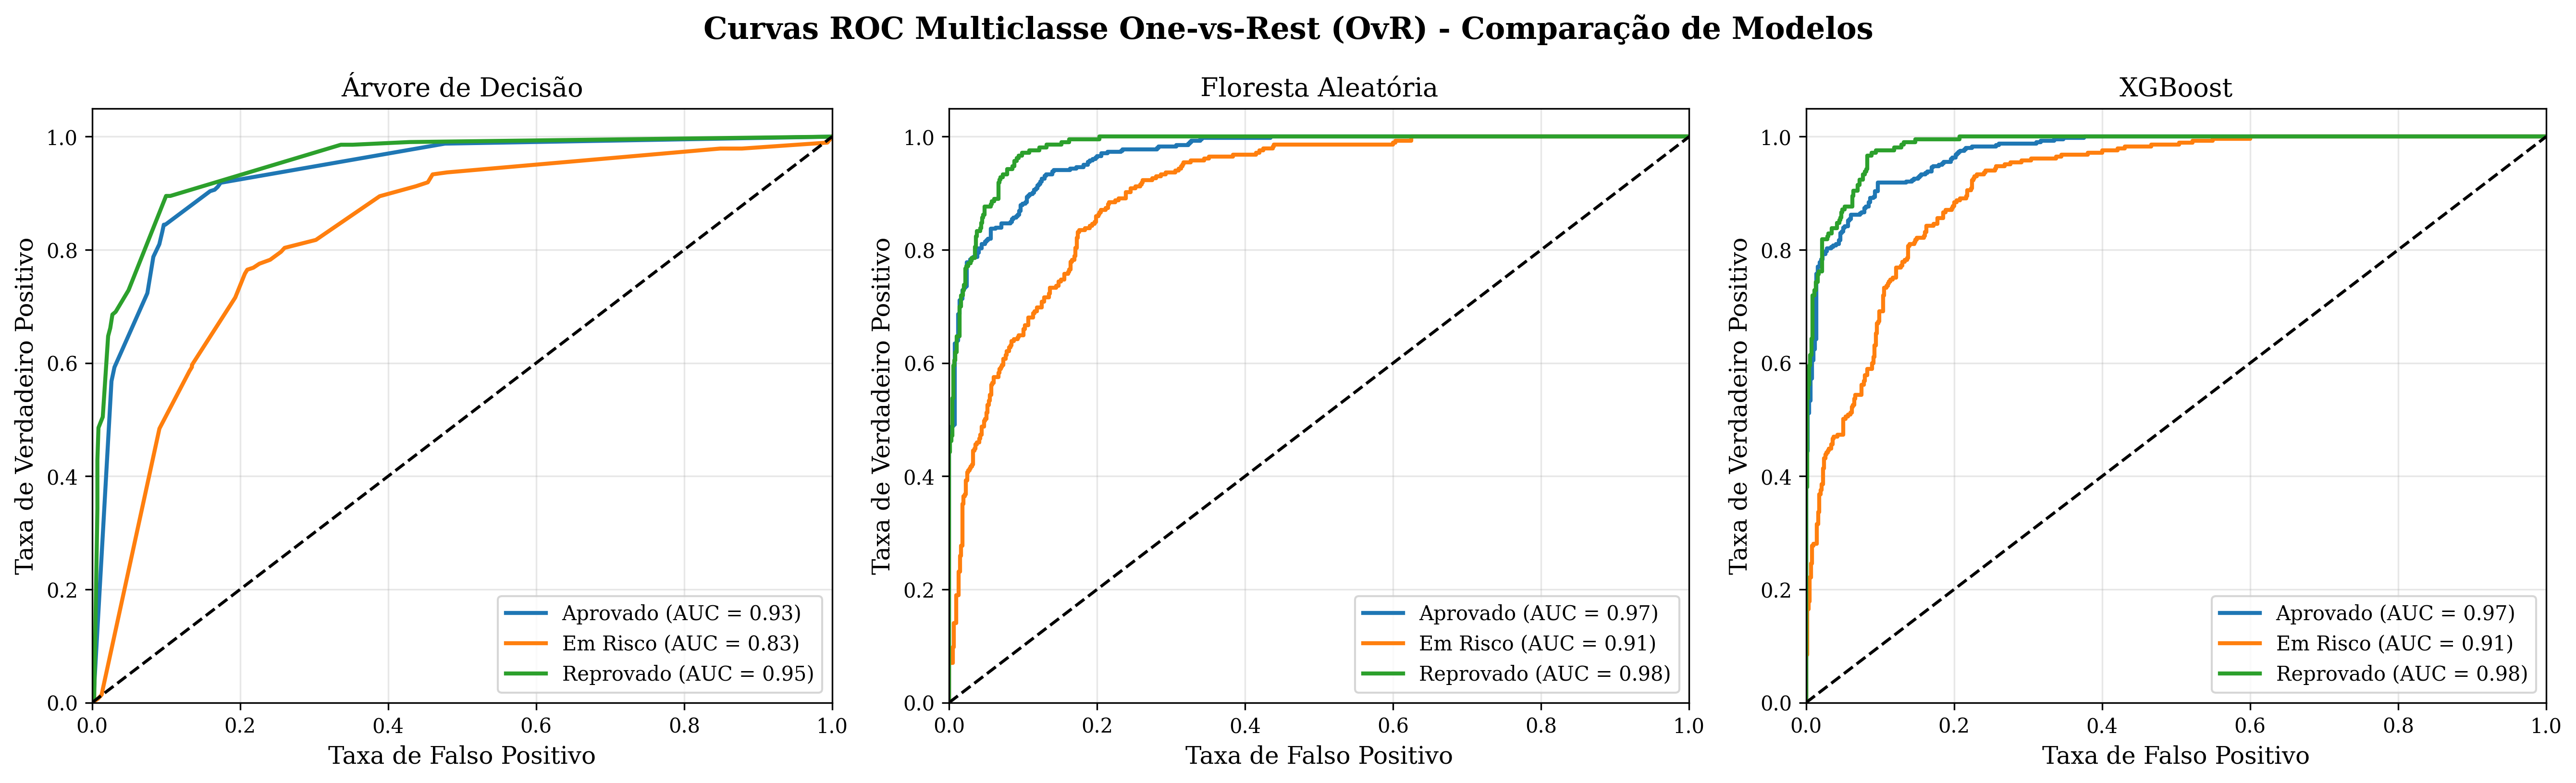
\includegraphics[width=0.98\textwidth]{imagens/roc_curves_comparison.png}
\source{Elaborado pelo autor (2026).}
\end{figure}

No XGBoost, as classes extremas apresentaram excelente separabilidade (AUC de 0,971 para \textit{Aprovado} e 0,983 para \textit{Reprovado}), enquanto a classe intermediária \textit{Em Risco} registrou AUC de 0,915. O mesmo padrão repete-se nos demais modelos (\textit{Decision Tree}: 0,932 / 0,827 / 0,951; \textit{Random Forest}: 0,968 / 0,905 / 0,981, na ordem Aprovado / Em Risco / Reprovado). A menor separabilidade da classe intermediária é esperada e estruturalmente explicável: ela ocupa a banda de fronteira da rotulagem, comprimida por duas fronteiras de decisão simultâneas, e os estudantes próximos aos limiares da LDB compartilham perfis observáveis com as classes vizinhas. Do ponto de vista pedagógico, o desempenho elevado na classe \textit{Reprovado} (\textit{recall} de 84,3\% no XGBoost, com precisão de 87,6\%) é o resultado mais relevante: o modelo raramente deixa de sinalizar o estudante em vulnerabilidade acadêmica severa, minimizando os falsos negativos que mais comprometeriam intervenções preventivas.

\section{Estudo Detalhado das Classes via Matriz de Confusão}

Para investigar a origem granular dos erros de predição, elaborou-se o mapa de calor das matrizes de confusão (Figura~\ref{fig:confusion_comparison}).

\begin{figure}[htb]
\centering
\caption{Matrizes de confusão obtidas nos ensaios de \textit{holdout} (teste).}
\label{fig:confusion_comparison}
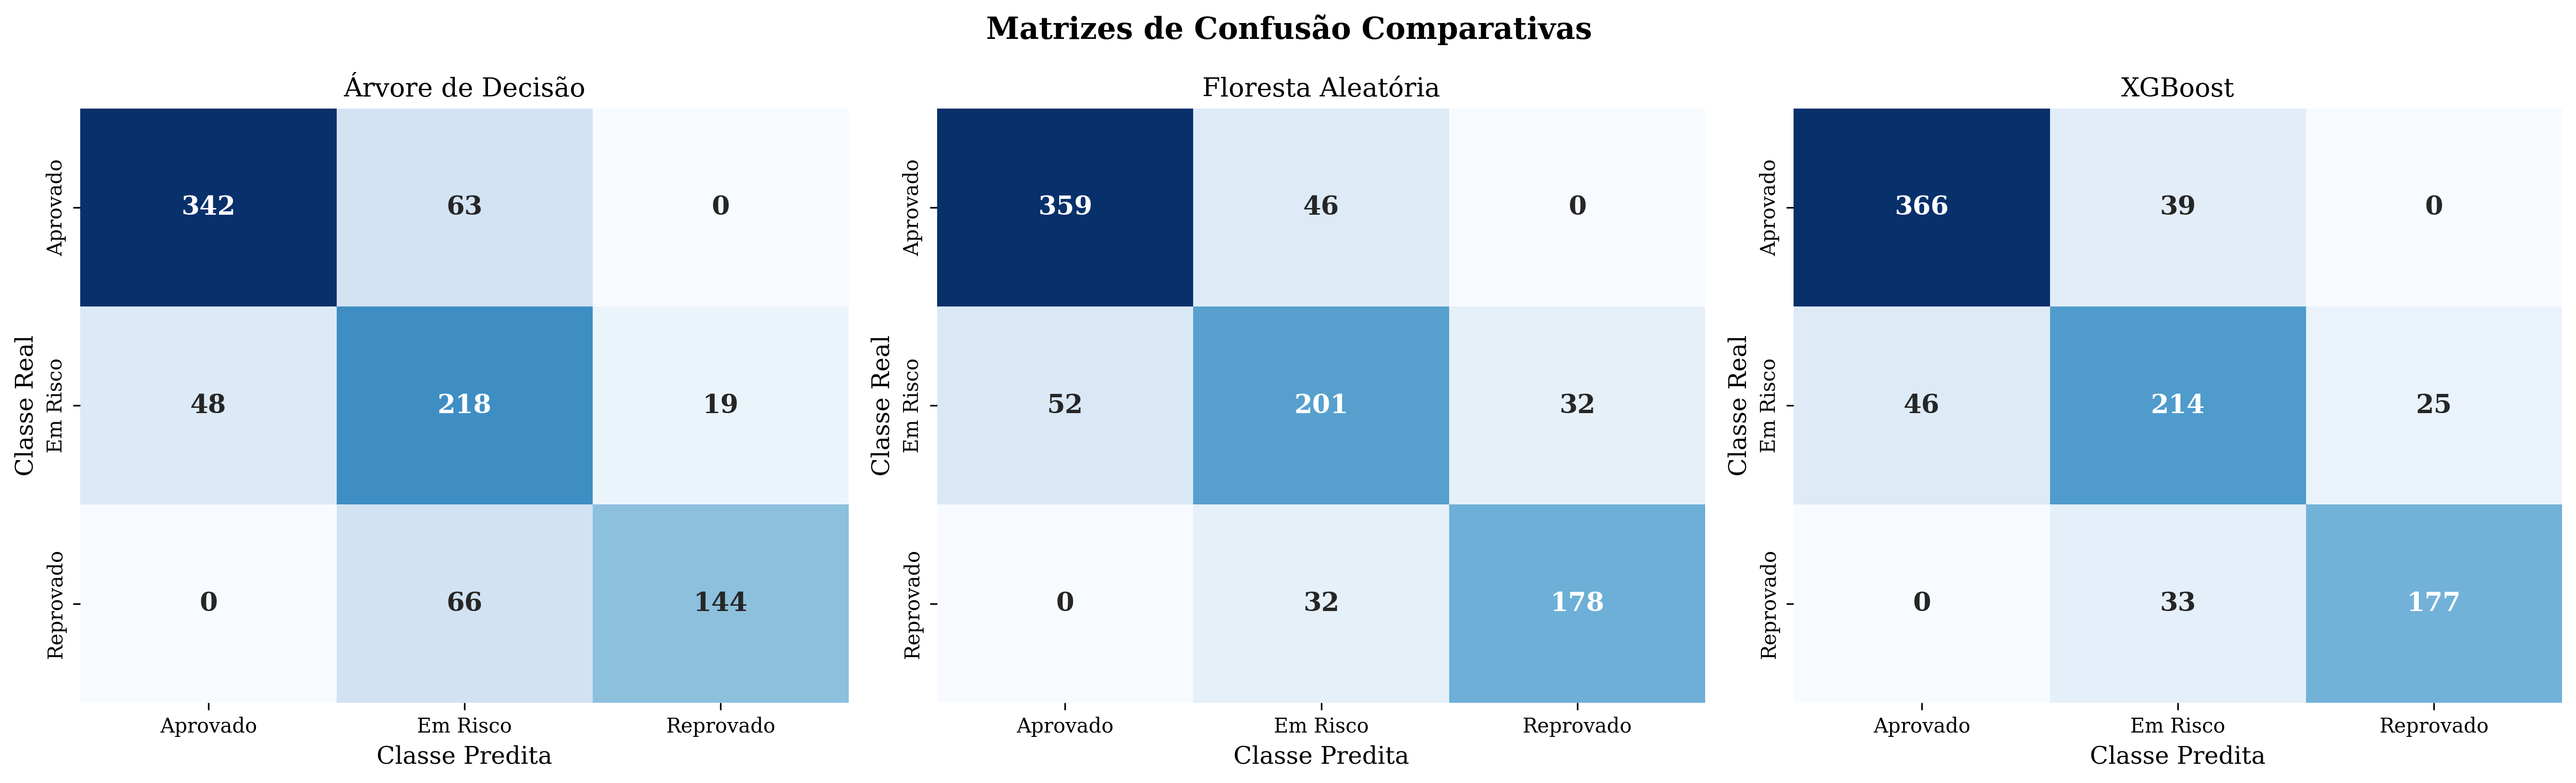
\includegraphics[width=0.98\textwidth]{imagens/confusion_matrices_comparison.png}
\source{Elaborado pelo autor (2026).}
\end{figure}

O achado mais significativo é a \textbf{ausência total de erros entre classes extremas} nos três modelos: nenhum estudante \textit{Aprovado} foi classificado como \textit{Reprovado}, nem o inverso. Todos os erros concentram-se em adjacências ordinais (\textit{Aprovado} $\leftrightarrow$ \textit{Em Risco} e \textit{Em Risco} $\leftrightarrow$ \textit{Reprovado}), o que indica que os classificadores capturaram a ordinalidade latente da tendência de desempenho. No XGBoost, dos 143 erros cometidos em 900 instâncias de teste, 85 ocorreram na fronteira \textit{Aprovado}--\textit{Em Risco} e 58 na fronteira \textit{Em Risco}--\textit{Reprovado} (erros de gravidade operacional reduzida, pois deslocam o estudante para uma categoria vizinha de atenção, sem inverter o prognóstico).

\section{Análise Dimensional e Importância dos Atributos}

A sustentabilidade ética e científica de intervenções educacionais assistidas por aprendizado de máquina exige interpretabilidade. A Figura~\ref{fig:feature_importance} apresenta as contribuições relativas dos atributos em cada classificador.

\begin{figure}[htb]
\centering
\caption{Critério de importância relativa dos atributos na predição de desempenho.}
\label{fig:feature_importance}
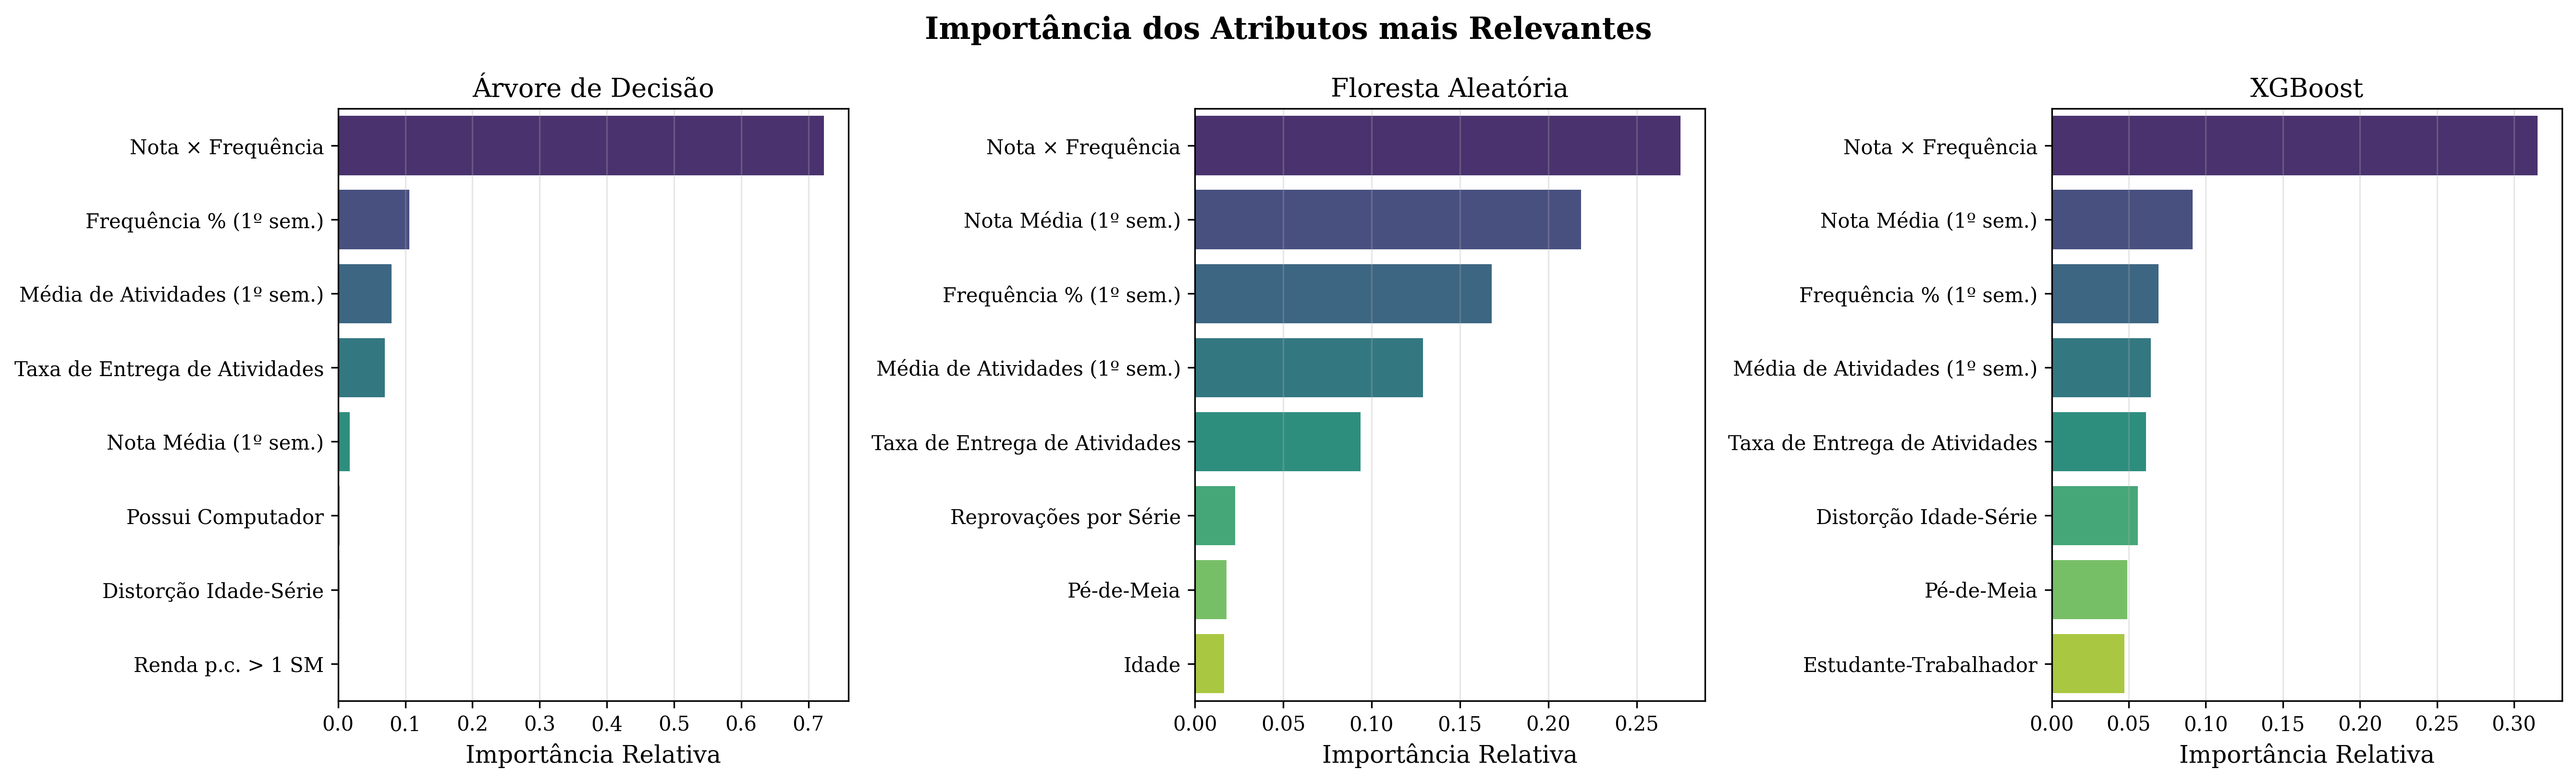
\includegraphics[width=0.98\textwidth]{imagens/feature_importances_comparison.png}
\source{Elaborado pelo autor (2026).}
\end{figure}

A variável derivada de interação nota--frequência (\texttt{nota\_x\_frequencia}) consolidou-se como o preditor de maior relevância em todas as estruturas (cerca de 72\% na \textit{Decision Tree}, 28\% na \textit{Random Forest} e 32\% no XGBoost), corroborando a literatura educacional: nota e frequência não operam isoladamente, mas de maneira sinérgica na representação do rendimento discente \cite{curi2006}. Na sequência aparecem os demais sinais acadêmicos parciais, incluindo as variáveis de engajamento contínuo introduzidas neste trabalho: no XGBoost, a média das atividades responde por 6,4\% e a taxa de entrega por 6,1\% da importância (evidência de que a regularidade do engajamento agrega informação além da nota média e da frequência, em linha com a literatura de EDM \cite{costa2012, fredricks2004}).

O resultado central para a questão de pesquisa, contudo, está na camada seguinte de importâncias do XGBoost: os \textbf{fatores sociológicos} dominam as posições subsequentes: distorção idade-série (5,6\%), recebimento do Pé-de-Meia (4,9\%), trabalho juvenil (4,7\%), renda \textit{per capita} de até meio salário mínimo (3,5\%) e acesso à internet (3,1\%). Cumpre interpretar esse achado nos seus devidos termos: como o fenômeno gerador é sintético, ele não constitui evidência empírica independente de que tais fatores condicionam o desempenho real (essa relação é premissa do gerador, fundamentada na literatura sociológica \cite{berlato2020, marturano2015}). O que o resultado demonstra é de natureza \textbf{metodológica}: os classificadores foram capazes de \textit{recuperar}, a partir exclusivamente dos atributos observáveis, o peso não redundante que os fatores sociológicos receberam no fenômeno gerador, mesmo na presença de indicadores acadêmicos diretos, o que confirma a hipótese H2 e valida a capacidade da arquitetura de capturar essa estrutura quando ela existir nos dados. A posição de destaque do indicador de assistência financeira, em particular, mostra que o modelo capturou o efeito de reversão de tendência do Pé-de-Meia embutido nas regras de geração, cuja fundamentação está na literatura \cite{santos2026}.

Por fim, ressalta-se a salvaguarda anti-viés: gênero e cor/raça foram gerados com peso zero no fenômeno e excluídos do treinamento, juntamente com a origem escolar, de modo que nenhuma decisão do modelo se apoia em atributos demográficos protegidos, uma decisão alinhada às boas práticas de equidade algorítmica em contextos educacionais. As limitações que condicionam a leitura desses resultados são discutidas, em conjunto com suas implicações, na seção de Limitações e Implicações das Considerações Finais.
